\documentclass[a4paper,11pt]{article}
\usepackage[osf]{mathpazo}
\usepackage{ms}
\usepackage[]{natbib}
\raggedright

\newcommand{\datastorr}{\texttt{datastorr}}
\newcommand{\smurl}[1]{{\footnotesize\url{#1}}}
\newcommand{\ghsmurl}[1]{{\footnotesize\href{https://github.com/#1}{#1}}}

\usepackage{graphicx}

\title{Versioned data: why it is needed and how it can be achieved (easily and cheaply)}
\author{Daniel S. Falster$^{1,*}$, Richard G. FitzJohn$^2$,\\ Matthew
  W. Pennell$^3$, and William K. Cornwell$^{1}$}
\affiliation{
$^1$ Evolution \& Ecology Research Centre, School of Biological, Earth and Environmental Sciences,
University of New South Wales, Sydney, NSW 2052, Australia\\
$^2$ School of Public Health, Imperial College, London SW7 2AZ United Kingdom\\
$^3$ Department of Zoology and Biodiversity Research Centre,\\
University of British Columbia, Vancouver, B.C. V6T 1Z4 Canada\\
$^*$ Corresponding author: daniel.falster@unsw.edu.au\\
}
\date{}

\bibliographystyle{mee}

\usepackage[title,titletoc,toc]{appendix}

\mstype{Article Note}
\runninghead{Versioned Data Delivery}
\keywords{Data sharing, Version control, Semantic versioning, Meta-analysis}

\begin{document}
\mstitlepage
\noindent
\parindent=1.5em
\addtolength{\parskip}{.3em}
\doublespacing
\linenumbers


\section{Summary}

The sharing and re-use of data has become a cornerstone of modern science.  To help this process, numerous linked tools have been developed to allow quick and easy data sharing:    a data file for a particular analysis can be quickly uploaded, given a digital identifier, and shared.  Thus far, however, this framework does not accommodate on-going scientific progress: for many important problems, particularly those suitable for meta-analyses, datasets will continue to grow with time --- more data points will be added, and new and more useful data structures will be created.  Essentially this means that datasets, like science in general, improve with time.  We suggest that many different datasets would be more useful if organized as a series of versions, with a simple naming system to allow users to perceive the type of change between versions.  In this article, we argue that adopting the paradigm and processes for versioned data, analogous to software versioning, would be useful for both data curators and users of even small-to-medium sized datasets. We introduce a system called Versioned Data Delivery (\textsc{vdd}) and present tools for creating, archiving, and distributing versioned data easily, quickly, and cheaply. These new tools allow for individual research groups to shift from a static model of data curation to a dynamic and versioned model that more naturally matches the scientific process.

\section{Introduction}

As is evidenced in the advent of this journal \citep{Editorial-2014}, publication of quality datasets is now considered a first-class scientific product. Increasingly, funding bodies, publishers, and scientific social norms are recognizing the value of sharing data, including as standalone products without any accompanying analyses \citep[e.g.][]{Whitlock-2011,Fairbairn-2011,Piwowar-2011,VanNoorden-2013,Gibney-2013}. Datasets are now routinely archived as part of the publishing process. Moreover, increasing numbers of standalone ``Data papers'' (or descriptors) have been appearing in standard domain-level journals, as well as specialised data journals. Yet, while the last decade has witnessed a rapid and exciting change in attitudes towards data sharing and publishing, the scientific community is still grappling with how to effectively disseminate and manage open-source datasets \citep{Whitlock-2011, Goodman-2014, Lowndes-2017,Perkel-2016,VanNoorden-2013, Kratz-2015}. In particular, the current data publishing model has not yet embraced the idea that many  datasets are designed to answer scientific questions that extend beyond the scope of a single empirical paper.  These datasets are constantly evolving, i.e. they are never "finished", and may be the subject of repeated analysis or meta-analysis.

Many, and perhaps most, of the datasets published in \emph{Scientific Data} are likely to be living entities, meaning the state-of-the-art (or ``canonical'') version of the dataset will change through time. Typical changes include: the adding new data, improving the quality of existing data, integrating with other databases, or re-structuring the database content to be able to address new questions. For example, a dataset on a biological organisms might be expanded through the addition of new records or improved through the correction of spelling mistakes in taxonomic names. As research around a data product grows, there might be many such additions. Ideally, any changes to a dataset would become immediately available to any interested parties, while past versions of the dataset would remain accessible to ensure reproducibility.

However, current models for publishing datasets do not facilitate distributing successive versions of a dataset in an effective and scalable manner. The most common current working model for publishing scientific datasets is to archive them in a variety of open-source data repositories where the data is attributed a Digital Object Identifier (\textsc{doi}) -- such as \texttt{Dryad}, \texttt{Figshare}, or \texttt{Zenodo}. Publishing involves a single data deposition. And once published, datasets are immutable. That means that most published datasets exist as a singular snapshot of the dataset, taken at the time the data descriptor was published. While it might only require a small amount of work to update the dataset, if there is no way to distribute the updated dataset, then that work has to be re-done by every user of that dataset. Moreover, those required changes add steps between the canonical dataset and any analysis using it, making reproducibility of the new analysis more difficult than it needs to be. We refer to this type of data delivery as being ``Static'' (Table \ref{tab:publishing_models}).

Many research groups solve the issue of versioning data internally in a variety of ad hoc and suboptimal ways. A common solution is to email around the latest versions with version numbers appended to the filename. Another approach is to repeat corrections or updates that have been made elsewhere. Alas, these practices are both inefficient and a barrier to reproducibility, as the dataset used in a future publications may differ to the version previously made available on-line. There is therefore a strong need for an easy way to distribute changes to a dataset after its initial publication to potential users, along with notes on what has changed and why since the previous version.

In this article we
\begin{enumerate}
  \item Introduce the concept of Versioned Data Delivery (\textsc{vdd}).
  \item Outline how emerging technologies in data science (Table \ref{tab:technologies}) can be used to help researchers maintain, distribute, and access small-to-medium sized datasets.
  \item Introduce a new \textsc{R} package called \texttt{datastorr}, a proof-of-concept implementation of a \textsc{vdd} system.
\end{enumerate}
The issue of updating and expanding published data has already been addressed in large centralised repositories like genetic sequences (\texttt{GenBank}) or species location data (\texttt{GBIF}), where new data can be added and there exist abilities to correct errors in existing records (e.g. by adding multiple version of a genetic sequence). Yet these ``Dynamic'' web databases (Table \ref{tab:publishing_models}), require a level of infrastructure that is beyond most research groups. Our focus here is on the wide range of datasets, such as those appearing in this journal, that are not covered by these repositories. In most of these cases, the data collected will not be ``big'' but rather small-to-medium sized. Such data support important research projects on particular scientific questions, but are not, in most cases, general enough to warrant custom infrastructure. Further, while we emphasize particular technologies in our implementation, the principles are general and could easily be ported to other platforms.

\section{A lightweight, cheap, and scalable workflow for delivering versioned data}

In brief, the \textsc{vdd} workflow we present borrows best-practices for software development \citep{Perez-Riverol-2016} and applies them to the challenge of maintaining and distributing Versioned Data. Software developers maintain a core set of code which produces a binary executable file that can be installed on a users local computer. With a \textsc{vdd} system, data developers similarly maintain a core set of files (the ``code''), which produce an organised dataset that can be ``installed'' on a user's local computer. In either the development of software or data, successive versions are released over time (called ``releases''). The similarity in workflow between software and data then allows us to deploy the same technological platforms that are used in software development, for the development and distribution of data. Importantly, our \textsc{vdd} systems uses well-established tools (Table \ref{tab:technologies}), ensuring high-level performance and stability.

The core technologies used are summarised in Table \ref{tab:technologies} and described further below. Several groups will interact with the \textsc{vdd} system, including dataset \emph{maintainers}, \emph{contributors}, and \emph{users}. The requirements of these different groups are outlined in Table \ref{tab:user_requirements}.

\subsection{Version control}

Version control, primarily an open-source variety called \texttt{git}, has become ubiquitous in software development. In practice, version control tracks line-by-line changes in text files and creates and maintains a history of those changes. Increasingly version control has been applied to scientific code and data management, especially for small-to-medium sized datasets \citep{Ram-2013, Perkel-2016, Lowndes-2017}. \texttt{git} is attractive for data management because it tracks all changes in monitored files, provided these are saved in text format (e.g. ``.csv'', ``.tsv'', ``.txt''). The history is visible to anyone interacting with the repository. It also allows users to annotate changes (``commits'') with informative messages detailing the rationale for those changes. In it's present form, \texttt{git} can handle individual data files at least up to 100MB, which includes a large fraction of scientific cases.

As a general strategy for tracking a dataset under version control with git, we recommend:
\begin{enumerate}
  \item Dataset \emph{maintainers} establish a separate \texttt{git} repository for any dataset to be distributed.
  \item Saving all files as plain text, so that \texttt{git} can identify line-by-line changes. For example, you might maintain tabular data as a ``csv''.
  \item Saving data in their rawest form. In some datasets you might only have a single file. Others may have may files that get manipulated or combined in some way to produce a unified product.
  \item Including in the \texttt{git} repository any code needed to manipulate or compile the raw data files into the final dataset. For example, you might combine many independent datasets into one unified dataset.
  \item Documenting any change in the dataset as a ``commit'' into the \texttt{git} repository logs, with informative commit messages outlining why a particular change was made.
\end{enumerate}

\subsection{Hosting and distributing versioned data}

Datasets stored under version control via \texttt{git} reach their real potential when hosted at a suitable internet hosting service \citep{Ram-2013,Perkel-2016}. Here we focus on the platform \texttt{GitHub} (Table \ref{tab:technologies}), but similar functions could be achieved via other providers such as \href{http://bitbucket.org}{bitbucket.org} and \href{http://gitlab.com}{gitlab.com}. Hosting of a \texttt{git} repository enables dataset \emph{maintainers} to connect with other potential \emph{contributors} and also \emph{users} (Fig. \ref{fig:technology_stack}). These platforms are designed to work with \texttt{git} repositories, and thus offer many helpful features, such as ability to record issues, host documentation, or review edits over time.

Of particular interest for current purposes, is \texttt{GitHub}'s ability to host a stream of ``releases'' from the dataset, alongside the \texttt{git} repository containing all the rawfiles. Each ``release'' is linked to a specific commit in the \texttt{git} repository history and occur at points where the dataset \emph{Maintainer} decided to generate a new  version of the data for distribution. While \emph{users} could in principle download the entire \texttt{git} repository, actually all they want are these 'releases'.

Deciding when to make a new release is at the discretion of the dataset \emph{Maintainer}. In practice, one makes fewer releases than one does commits into the \texttt{git} repository, though there is nothing stopping \emph{maintainers} from releasing a new version for every commit. The flexibility here allows \emph{maintainers} to do internal work between releases and only \emph{release} the data to users when the revision represents a clear improvement on the previous release.

Another important consideration is that websites like \texttt{GitHub} naturally cater for two types of data users to access the data: those that interact with the data via point and click downloading and those that use programmatic interaction (Fig. \ref{fig:technology_stack} and Table \ref{tab:user_requirements}). Specifically, \texttt{GitHub} releases can be downloaded directly by users via point-and-click, or accessed programmatically via the \texttt{GitHub} \textsc{api}.


\subsection{`Semantic' versioning}

To realize the full benefits of a versioned controlled dataset, users should be able to easily intuit the types of changes that have occurred among versions. Since software development has effectively already dealt with almost identical; problem in the labelling of software releases, we suggest there is benefit in adopting the best-practices from that field.

Specifically, we suggest applying the theory of ``semantic versioning'', developed for software distribution (see \href{http://semver.org/}{semver.org}), to successive releases of a dataset. Semantic versioning uses tri-digit notation of the form ``X.Y.Z'' for successive versions, where X, Y, and Z are non-negative integers. For example, version ``1.0.0''. Changes in the version number then signal the type of changes that occurred in the dataset (Fig \ref{fig:semantic}). Applying semantic versioning to data, a change from:
\begin{itemize}
  \item  {\bf 1.0.0 $\rightarrow$ 1.0.1}: implies a {\bf correction} or ``patch'', for example a small error correction which is unlikely to ``break'', or change in a substantial way, a users' analyses, although there may be minor changes in the results.
  \item {\bf 1.0.0 $\rightarrow$ 1.1.0}: implies a {\bf minor} enhancement, for example adding a new study to a meta-analysis dataset (while otherwise maintaining the same dataset structure); this change is large enough that in the view of the database curator it might change the results of some users' analyses.
  \item {\bf 1.0.0 $\rightarrow$ 2.0.0}: implies a very {\bf major} revision, for example improving the entire structure of the dataset and adding new columns. These changes are very likely to change the results of most users' analyses or to break code that was written to work on the previous version of the database or both.
\end{itemize}
Any user of a dataset where releases were tagged using semantic versioning, would immediately know the types of change that might have occurred when requesting different versions and set their there expectations accordingly.

% I think that major version increments could still be looked at as
% _breaking_ changes as often as large additions of data.  Changing
% column names, removing columns, changing the structure of linked
% tables etc.

\subsection{\texttt{datastorr} and dataset-specific \texttt{R} packages}

To aid reproducibility and efficient usage, many users will want access to all versions of any particular dataset programmatically (Table \ref{tab:user_requirements}). Code to access a stream of \texttt{GitHub} releases could be written individually by each user, but this creates an unnecessary technological hurdle. To make it easier for users to access Versioned Data via code, we offer a novel implementation of \textsc{vdd} focussing on the \texttt{R} platform, as one of the most prominent platforms for data science \citep{R-2017}.

Here we introduce a dedicated \textsc{R} package, called \texttt{datastorr} (\smurl{github.com/richfitz/datastorr}), that facilitates access to releases of any Versioned Data hosted on \texttt{GitHub} (Fig. \ref{fig:technology_stack}). Specifically, the  \texttt{datastorr} package:
\begin{enumerate}
  \item Constructs the shell of a second, dataset-specific \textsc{R} package, which is used to access releases from a specific repository stored on \texttt{GitHub};
  \item Contains the main code needed to interact with the \texttt{GitHub} \textsc{api} to retrieve versions of the dataset.
\end{enumerate}
Using \texttt{datastorr}, a researcher can create and distribute a custom \textsc{R} package that facilitates access to their data with (very) minimal computational skills.

For example, \texttt{datastorr} was used to build the package \texttt{baad.data} (\smurl{github.com/traitecoevo/baad.data}), which is an interface to the Biomass and Allometry Database (\textsc{BAAD}) \citep{Falster-2015} stored at \smurl{github.com/dfalster/baad}. The R package \texttt{baad.data} consists of only a few simple functions and associated help files, that were automatically generated with \texttt{datastorr}. For a user, accessing a version of the data is a simple as typing a single line of code (Fig. \ref{fig:technology_stack}). Accessing a different version of the data involves changing only the version number. From the users perspective, the existence of the \texttt{baad.data} and \texttt{datastorr} packages makes reproducing analyses using specific versions of the data possible \citep[e.g.][]{Duursma-2016,Falster-2016}.

Using \texttt{datastorr}, dataset \emph{maintainers} can set up their own R package to deliver there versioned dataset simply by providing:
\begin{enumerate}
  \item a \texttt{GitHub} repository name (e.g., ``traitecoevo/baad.data'') where releases are stored;
  \item the filename in the release that will contain the Versioned Data;
  \item the function used to load this into \texttt{R}.
\end{enumerate}
A full tutorial explaining precisely how to set this up is available at \smurl{github.com/ropenscilabs/datastorr}.

Then as the dataset grows over time, the \emph{maintainers} update the \texttt{git} repo and create a \texttt{GitHub} release with a new version number. All the releases are simultaneously available to any user, both point-and-click and programmatically.

The dataset-specific packages created by \texttt{datastorr} are designed to be computationally efficient and also work offline. Packages created by \texttt{datastorr} contain no actual data, only the rules for fetching the data. As such, the basic package structure is quick to install and takes up virtually no space on the user's hard-drive. The package functions by fetching each data version once (the first time it is requested), and then caching these files locally for future reuse. Moreover, \emph{users} can have several versions of the same dataset on their computer and unambiguously access the different versions with one simple function call.

\section{Discussion}


% General problem. An example of solution. Key features

% The introduction talks at length about medium sized data and little about versioning but this section talks only about versioning
% WKC: now intro is about versioning and data size issue discussion moved here, which I think is an improvement


% Discuss Genbank or other large sites?
% The issues in practically doing the versioning are more acute when the
% data are bigger than small, that's all.

% From intro:
% When considering the right tool to store and deliver versioned data, the size
% of the dataset is another essential consideration. ``Big data'' brings with it
% specific needs and so requires a specific set of hardware and software tools.
% Examples of big data include genetic datasets, global datasets of species
% observations, and remote sensing data. This size of this data is bigger than
% that which individual research groups can maintain and often requires a
% specialized governmental or non-governmental institution with full-time staff
% to curate and maintain those research resources.


%work on this paragraph more
We acknowledge that the issues we have identified in this article will not come as news to most readers: datasets are constantly improving and, despite tremendous advances in data sharing and associated technologies over the last decade, there is little consensus about what to do with this fact. In some individual cases, such as \texttt{GenBank} (see \url{https://www.ncbi.nlm.nih.gov/genbank/sequenceids/}), researchers have thought about versioning and developed specific solutions. But so far these as we mentioned above, these datasets tend to be those managed by large, well-funded institutions or consortia and involve standard data types (e.g., sequences). But for an individual research group working with a specialized type of data, creating their own \texttt{GenBank} is clearly a non-starter. As a result, we argue that there is a substantial need for a easy, cheap, and flexible solution and suggest that adopting a \textsc{vdd} system may be one way forward.

% Moved from above, need to integrate better
We have created \texttt{datastorr} to make \textsc{vdd} easy to implement and manage for \texttt{R} users. And as we stated above, this has already been used to release a variety of datasets (Table \ref{tab:examples}).
% Reword next senetnce
But the design choices we made in \texttt{datastorr} represent only one of many possible ways to adopt a \textsc{vdd} system; we can imagine many alternative models for interacting with \texttt{GitHub} (or an entirely different service and technology) and accessing versioned data programmatically.  The key is not the specific technology, but rather the concept of creating, maintaining, and distributing versioned data.

Many of the key roadblocks preventing a switch from a static to a dynamic data world were technological: in the past, it took great deal of money and expertise to set up and maintain a \textsc{vdd} system, but now there are many platforms for storing and distributing versioned controlled data with little or no cost.  The website \texttt{GitHub} (\smurl{www.github.com}) is a commercial platform for hosting and interacting with \texttt{git} repositories. In practice, each dataset should be a separate \texttt{git} repository on \texttt{GitHub} (see Table \ref{tab:examples} for examples). Although mainly used for computer code, \texttt{GitHub} is now also being use to manage scientific data \citep{Perkel-2016}. Maintaining the version controlled data in the cloud has two main benefits: first, it provides a platform for multiple data contributors to sync their files and correspond about changes in the dataset, and second, it hosts a stream of data releases, thus acting as a central point for  the collection, curation, and distribution of the data.  The proliferation of cloud-based tools and open-source software have now reduced these roadblocks considerably.  We argue that by linking together the tools described above, researchers can now produce, curate, and distribute Versioned Data much more easily and cheaply than in the past.

%The key features of a \textsc{vdd} system that are already possible are a versioning system to communicate small and large changes to users, both point-and-click and programmatic access to all versions, reliable distribution to many users, and stable, organized \textsc{doi}s (see Fig. \ref{fig:technology_stack}).  Moreover, it is relatively easy to update and add new versions.  Technology is moving forward rapidly and so it is very likely that the particular tools we describe above will add features and be even easier to use.  But, nonetheless, workable systems are already possible.

Additionally, one of the greatest benefits of using a cloud-based tool for development of open-source software has been the way it encourages contributions from multiple individuals working simultaneously, and even individuals from outside the initial group of project participants \citep{Rogers-2013}. Multiple users can make changes to different parts of the code (or in our case, data) and the \texttt{git} system will integrate these together (if that is possible) or, when needed, flag where there are conflicts that need to be resolved. As a result adopting a \textsc{vdd} system has the added benefit of facilitating collaboration among research groups.

%Systematically archiving data is a key part of good workflow \citep{Wilkinson-2016, Piwowar-2011, Whitlock-2011}, and tools for creating and archiving digital objects have seen rapid progress in recent years.  At present, each version of the dataset can be automatically archived and assigned a \textsc{doi}, via several providers (Table \ref{tab:doi_minting}).  Here we describe the particular integration of \texttt{GitHub} and \texttt{Zenodo}.  It is useful to have the ability to either be specific---reference a particular version for the purposes of reproducibility or general--reference the entire project.  \texttt{Zenodo} currently automatically supplies both ``concept'' and ``version'' \textsc{doi}'s to the commits associated with \texttt{GitHub} releases automatically \citep[Fig. \ref{fig:semantic} and ][]{Nielsen-2017}.  This allows users to very precisely reference either generally or specifically, both of which may be appropriate in different situations.

% I'm unclear on the precice benefits of dois here (and actually in
% general to a point); some further clarification might be useful.  So
% far as I know they are useful because (a) journal urls are terrible
% and inconsistent (b) because everyone has them.  I don't really know
% why else you'd need one.  Especially in our case we offer no promise
% of persistence (deleting the github repo would break the doi and we
% could update the repo to include different data trivially).  So what
% is being added?  Our retrival system does not use the doi at all!

% WKC: hmmmm not sure we've nailed this yet, see
% https://github.com/traitecoevo/data_versioning/issues/10#issuecomment-317059819

% subsection only temporary as not allowed by journal guidelines.
% trick is to say something about how things are getting better rapidly, but not scare people away from doing this now.  
\subsection{Future directions}

Technology for data management and distribution is moving forward rapidly.  The workflow we describe above works well with current tools and should work even more quickly with its future replacement.  Here, we highlight a few rapidly developing future tools that researchers should be aware of.

Because \texttt{git} was built for tracking changes in code, there are aspects of how it behaves that are not natural to apply to  data \citep{Perkel-2016}.  For example, because it tracks changes line-by-line rather than cell-by-cell, there are inefficiencies in how the software stores the changes.
There is rapid current work on new implementations which will be faster computationally, smaller in file size, flexible with respect to data structures, and thus allow for larger datasets to be versioned efficiently \citep{Fli, Dat}.
% Add CKAN, rdrop2 and Git-LFS, conceptually at least, and say something useful about the future

Another area requiring attention is properly allocating credit to authors for these citations, and we hope that the large citation mapping services (\texttt{Web of Science} and \texttt{Google Scholar}) will adapt to the community standard once the research community settles on best archiving practices for versioned data. Likewise, we are optimistic that our funding bodies, research institutions, and scientific colleagues will further recognize the value in adding to, improving, and curating existing datasets in addition to collecting new ones.


% We have constant drama at work because the different spreadsheet
% writers we use across the platforms quote files inconsistently so
% every save is a complete rewrite of the file.  It's totally
% impossible to do any collaborative editing....
% For open-source projects, external parties are also welcome to copy (in \texttt{git} speak ``clone'' or ``fork'') a repository, make their own modifications and send these back to the project \emph{maintainers} to be reviewed and potentially included in the project. This process is called submitting a ``Pull request''. One of the potential advantages of moving the workflow for managing data onto \texttt{GitHub} is the potential for seamless collaboration and for receiving pull requests from contributors \citep{Perkel-2016}.
 % This section conflates git and github more than is useful.  It
 % might be worth setting up github as the explicit platform here or
 % dialing back the language a bit.  GitLab and bitbucket have their
 % own "merge request" feature (I think).  It's also github that makes
 % repositories _discoverable_ which is a requirement for getting
 % outside collaborators in.  Oddly the decentralised nature of git is
 % not actually that useful in the github model because github is so
 % strongly centralised.  Will and I did some true decentralised git
 % collaboration on a plane to nescent once with a bare git repo on a
 % thumb drive.


% So, git doesn't actually work this way, though everyone seems to
% think that it does.  Git stores *content* and then later tries to
% de-duplicate it.  It then displays changes as line-by-line diffs
% (but you can change this to display the changes other ways; see
% --color-words --ignore-all-space for example.  The problem is that
% the algorithms that git uses are optimised for typical sizes of code
% and not for data.  Small data is actually totally fine to store with
% git.  The other issue that turns up is if the files are _binary_
% then an arbitrarily small change in the underlying data can result
% in an arbitrarily large change in the binary representation, which
% prevents deduplication.
%
% Git-LFS tries to step around this by storing large files separately
% from git's general machinery.  Git-annex did the same.  But they
% suffer from some of the other issues with git which are that it's a
% bit of a pain for (especially novice) users to do nontrivial things
% with.  I _always_ have to look up how to compare two versions across
% branches.  And there's no simple way of loading in two versions of
% the data into R without ending up with two working copies or doing
% some nasty "git show" call.

% I really think that something like CKAN (though it doesn't support
% holding data if I remember correctly) could totally be a complete
% solution to the sorts of issues that we have here.

% Karthik has started with rdrop2 again I think; I do think that is a reasonable low-entry way of distributing things


% Dan Noble: I think this is a pragmatic view, but I would have a tendency not to discuss how the tools you can use for a VDD approach are likely to be "replaced in the near future”. Of course, things change, but this will not entice the people you want the paper to appeal to to adopt this sort of approach. From my experience, some of the resistance to adopting this stuff comes from programs or repositories being “replaced” at such a high rate. They just don’t feel like its worth doing.

\section{Acknowledgements}
We thank D Noble for comments on an earlier draft and C Boettiger  for helpful discussions. DSF was funded by the Australian Research Council. MWP was funded by a NSERC Discovery Grant.

\newpage

\section{Tables}

\begin{table}[h!]
\centering
\caption{Alternative frameworks for setting up and managing a living database}
{\footnotesize
\vspace{1cm}
  \begin{tabular}{p{2.5cm}p{3.5cm}p{3.5cm}p{4cm}}
  \hline
  \textbf{Feature} & \textbf{Static datasets}& \textbf{Web database} & \textbf{Versioned data delivery}\\
  \textbf{} & (e.g. \smurl{datadryad.org})& (e.g. \smurl{coraltraits.org}) & (eg. \texttt{datastorr} via \texttt{GitHub})\\
  \hline
   Webserver        & bespoke & bespoke &  \smurl{github.com}\\
   Backend          & none & SQL + Ruby-on-rails 			& \texttt{git} + \texttt{datastorr} \\
   User access      & Web browser & Web browser 				    & Web browser or R \\
   Ease of setup    & Very easy & Hard 							& Easy\\
   Data size        & Up to several Gb & Small-Very large 				& Up to 1Gb\\
   Cost             & Varies & Varies  						& Free \\
   Bandwidth        & Managed by provider & Pro rata 						& Managed by \texttt{GitHub}\\
   Maintainer skills & None & Ruby + php 					& R + \texttt{git} \\
   User skills      &Web browsing& Web browsing  					& basic R \\
   Versioning       &None& Hard 							& Easy \\
   \textsc{doi} minting      &Automatic & Manual 					& Automatic \\
  \hline 
  \\
 
  \end{tabular}
  } 
\label{tab:publishing_models}
\end{table}

\newpage

\begin{table}[h!]
\centering
\caption{Overview of technologies used to maintain, store, and distribute the Versioned Data as described in this paper.}
{\footnotesize
\vspace{1cm}
  \begin{tabular}{p{5cm}p{10cm}}
  \hline
  \textbf{Technology} & \textbf{Description} \\\hline
  \textsc{API}   & An Application Programming Interface provides a set of protocols for exchanging information.\\
%   \textsc{CRAN}  &  Open source repository of packages for the R language \\
   \texttt{datastorr} & R package used to fetch versioned releases from \texttt{GitHub}  \\
   \textsc{doi} & Digital object identifier, which refers a user to a single digital object \\
%   \textsc{doi} ``minting'' & Allocation of a \textsc{doi} to a data product\\
   \texttt{git} & Open source version control system used for tracking progressive changes in a set of text files, typically computer code but also data\\
   github.com & A commercial web platform for sharing, visualising, and managing `git' repositories. Includes ability to browse the `history', `issue' tracking, and ability to create `releases'.\\
   \texttt{R}     &  Open source statistical and data processing language \\
   \hline
  \end{tabular}
  }
\label{tab:technologies}
\end{table}

\newpage

\begin{table}[h!]
\centering
\caption{Groups of users interacting with the Versioned Data Delivery system described and their requirements.}
{\footnotesize
\vspace{1cm}
  \begin{tabular}{p{2cm}p{5cm}p{7cm}}
  \hline
% Latex being the worst has made the overflow in the second column flow through to affect the third.  I used to know how to deal with this...
  \textbf{Group} & \textbf{Goal} & \textbf{Requirements} \\ \hline
  Maintainer & Create and distribute versioned datasets & Low technical overhead \\
    & & Easy workflow for releasing new versions \\
    & & Long term preservation \\
    & & Easy to crowd-source error checking and contributions \\
    & & Low initial cost \\
    & & Low on-going maintenance \\
  Contributor & Contribute to future versions of a dataset & Add new data \\
    & & Report errors in existing data  \\
  Users (all) & Easy access to releases from a versioned dataset & Introduction \& overview \\
    & & Long term stability \\
    & & Clear path for users to become contributors \\
  Users (programmatic) & Build reproducible products using specific versions of a dataset & Programmatic access to releases\\
    & & Easy installation\\
    & & Long term stability \\
  \hline
  \end{tabular}
}
\label{tab:user_requirements}
\end{table}

\newpage

\begin{table}[h!]
\centering
\caption{Example datasets using the Versioned Data Delivery system described in this paper.}
{\footnotesize
\vspace{1cm}

  \begin{tabular}{p{3.5cm}p{3cm}p{7cm}}
  \hline
   \textbf{\texttt{GitHub} repo} & \textbf{\texttt{R} package} & \textbf{Description} \\ \hline
  \ghsmurl{dfalster/baad} & \texttt{baad.data} & The \texttt{Biomass And Allometry Database} provides data on the size dimensions of plants for many species, compiled from multiple scientific papers \citep{Falster-2015}.\\
  \ghsmurl{traitecoevo/taxonlookup} & \texttt{taxonlookup} & Provides a taxonomic lookup table for land plants \citep{Pennell-2015a}.\\
  \hline
  \end{tabular}
  }
\label{tab:examples}
\end{table}

\newpage

\newpage


\begin{table}[h!]
\centering
\caption{Alternative platforms for minting \textsc{doi}s from \texttt{GitHub} repositories.}
{\footnotesize
\vspace{1cm}
  \begin{tabular}{p{4cm}p{8cm}}
  \hline
  \textbf{Provider} & \textbf{Features} \\ \hline
  \texttt{Zenodo}: \smurl{zenodo.org} & Automated \textsc{doi} for each \texttt{GitHub} release \\
    & Funded and maintained by CERN and OpenAIRE for long term preservation \\
    & At present, can only archive files embedded directly in the \texttt{git} repo, not produced by it as outputs\\
  \texttt{FigShare}: \smurl{figshare.com} & Builds data package based on \texttt{GitHub} release \\
    & Allows you to upload additional files, e.g. datasets built by code \\
    & Integrated with several journals, e.g. Nature family, \textsc{PNAS} \\
  \hline
  \end{tabular}
  }
\label{tab:doi_minting}
\end{table}

\newpage

\section{Figures}

\begin{figure}[!hb]
\centering
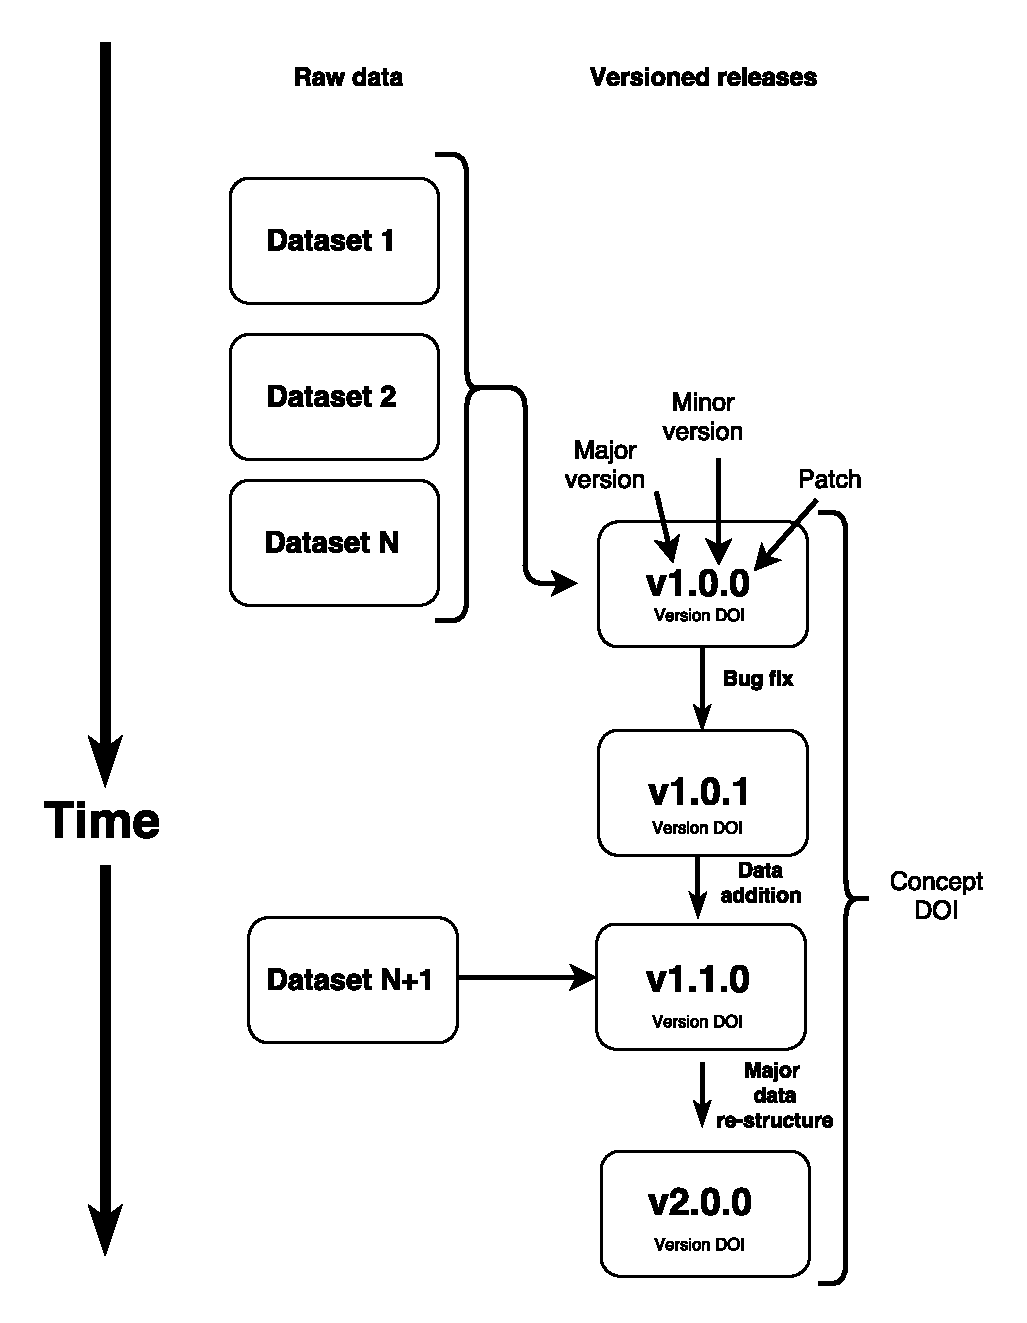
\includegraphics[width=\linewidth]{figures/Figure1.pdf}
\caption{
% could use a more descriptive legend. Maybe walk the reader through it a bit more. Also, I didn’t see (a) and (b) in that figure.
Semantic versioning allows users to anticipate the types of changes that have occurred between successive versions of a dataset.
\textbf{a)} 3 numbers indicate type of change.
\textbf{b)} A typical release stream.}
\label{fig:semantic}
\end{figure}

\newpage


\begin{figure}[!hb]
\centering
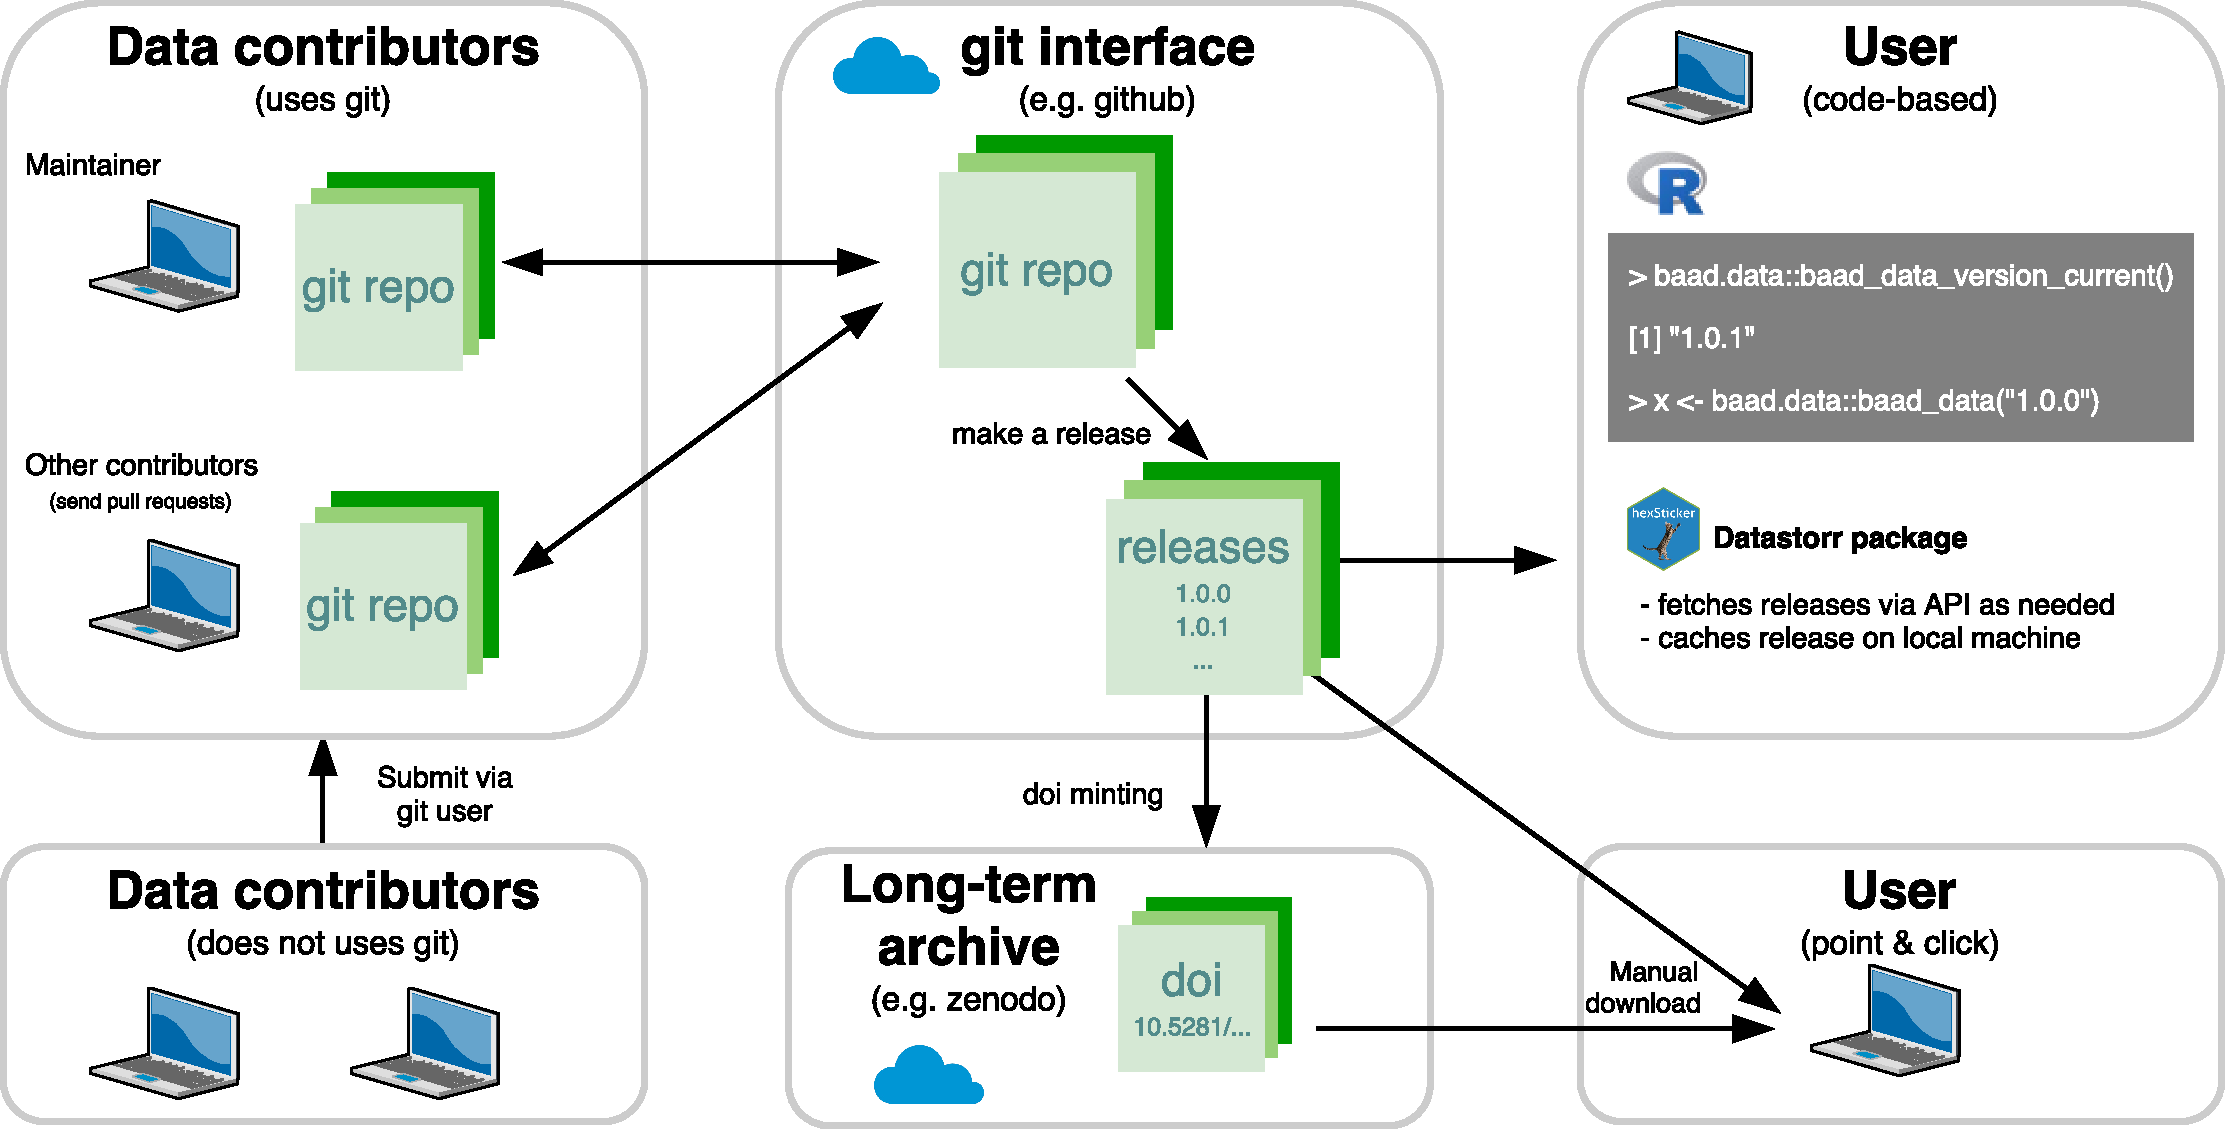
\includegraphics[width=\linewidth]{figures/Figure2.pdf}
\caption{Overview of the different users and technologies involved in distributing a versioned dataset via \texttt{datastorr}.}
\label{fig:technology_stack}
\end{figure}

\clearpage

\bibliography{refs}

\end{document}

